\begin{question}
\noindent In a Digital Art class, a student is designing a UI icon on a grid. Shape $P$ is transformed to shape $P'$, as shown on the grid below.

\begin{center}
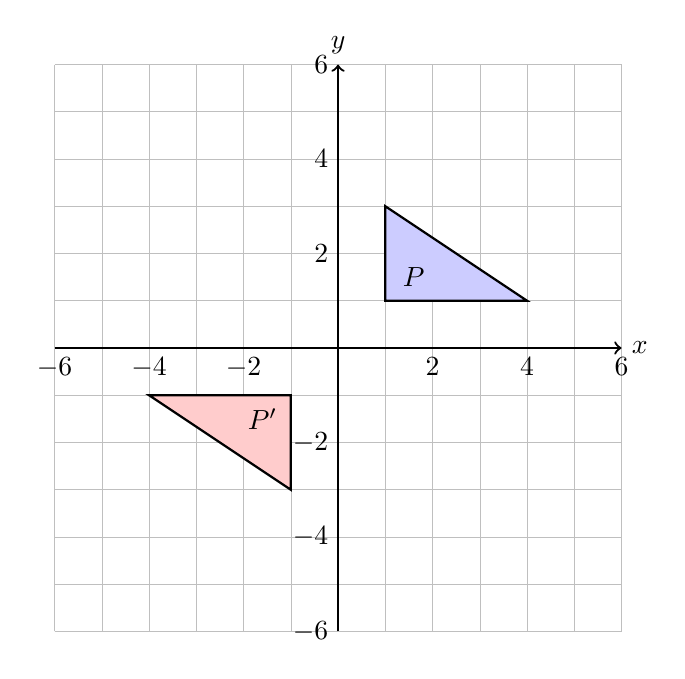
\begin{tikzpicture}[scale=0.6]
    \draw[step=1, lightgray, very thin] (-6,-6) grid (6,6);
    \draw[thick,->] (-6,0) -- (6,0) node[right]{$x$};
    \draw[thick,->] (0,-6) -- (0,6) node[above]{$y$};

    \foreach \x in {-6,-4,-2,2,4,6} \node[below] at (\x,0) {$\x$};
    \foreach \y in {-6,-4,-2,2,4,6} \node[left] at (0,\y) {$\y$};

    % Shape P: right-angled triangle with vertices (1,1), (4,1), (1,3)
    \draw[thick, fill=blue!20] (1,1) -- (4,1) -- (1,3) -- cycle;
    \node at (1.6,1.5) {$P$};

    % Shape P': rotated 180 degrees about origin -> vertices (-1,-1), (-4,-1), (-1,-3)
    \draw[thick, fill=red!20] (-1,-1) -- (-4,-1) -- (-1,-3) -- cycle;
    \node at (-1.6,-1.5) {$P'$};

\end{tikzpicture}
\end{center}

\noindent Shape $P$ has vertices at $(1,1)$, $(4,1)$ and $(1,3)$.\\
Shape $P'$ has vertices at $(-1,-1)$, $(-4,-1)$ and $(-1,-3)$.

\noindent Describe fully the single transformation that maps shape $P$ onto shape $P'$.

\vspace{4cm}
\begin{flushright}
    \answerlines{3}{3}
\end{flushright}
\end{question}